% arara: pdflatex
% !arara: biber
% !arara: pdflatex
% How to run: 
% 1) pdflatex "filename".tex
% 2) biber "filename"
% 3) pdflatex "filename".tex
% 4) pdflatex "filename".tex


\documentclass[x11names]{article}
\usepackage{verbatim}
\usepackage{listings}
\usepackage{graphicx}
\usepackage{a4wide}
\usepackage{color}
\usepackage{amsmath}
\usepackage{amssymb}
\usepackage[dvips]{epsfig}
\usepackage[T1]{fontenc}
% \usepackage{cite} % [2,3,4] --> [2--4]
\usepackage{shadow}
\usepackage{hyperref}
\usepackage{physics}
\usepackage{url}
\usepackage{tikz}
\usepackage{subcaption}
\usepackage[utf8]{inputenc}
\usepackage{booktabs} % Allows the use of \toprule, \midrule and \bottomrule in tables
\usepackage[font={small,it}]{caption}
\usepackage[margin=0.7in]{geometry} %Sets the margins in the document
\usepackage{siunitx}    %Allows use of SI units macros

%Defines calculator way to write powers of ten
\sisetup{output-exponent-marker=\textsc{e}}


% Change numbering and some commands
\renewcommand\thesection{Exercise \Roman{section}}
\renewcommand\thesubsection{\Roman{section}.\alph{subsection}}

%% references
\usepackage[style=authoryear,
            bibstyle=authoryear,
            backend=biber,
            % refsection=chapter,
            maxbibnames=99,
            maxnames=2,
            firstinits=true,
            uniquename=init,
            natbib=true,
            dashed=false]{biblatex}

\addbibresource{bibliography.bib}
% \addbibresource{top.bib}

% \bibliography{bibliography}
% \bibliography{top}


\usepackage[capitalize]{cleveref}

\setcounter{tocdepth}{2}

\lstset{language=c++}
\lstset{alsolanguage=[90]Fortran}
\lstset{basicstyle=\small}
\lstset{backgroundcolor=\color{white}}
\lstset{frame=single}
\lstset{stringstyle=\ttfamily}
\lstset{keywordstyle=\color{red}\bfseries}
\lstset{commentstyle=\itshape\color{blue}}
\lstset{showspaces=false}
\lstset{showstringspaces=false}
\lstset{showtabs=false}
\lstset{breaklines}


\definecolor{keywords}{RGB}{255,0,90}
      \definecolor{comments}{RGB}{0,0,113}
      \definecolor{red}{RGB}{160,0,0}
      \definecolor{green}{RGB}{0,150,0}
       
      \lstset{language=Python, 
              basicstyle=\ttfamily\small, 
              keywordstyle=\color{keywords},
              commentstyle=\color{comments},
              stringstyle=\color{red},
              showstringspaces=false,
              identifierstyle=\color{green}
              }



\title{ Exercise 4 \\ Sommerjobb Numeriske Plasmaoppgaver }
\author{Gullik Vetvik Killie	}


%%%%%%%%%%%%%%%%%%%%%%%%%%%%%%%%%%%%%%%%%%%%%%%%%%%%%%%%%%%%%%%%%%%%%%%%%%%%%%%%%%%%
% Actual text starts here
%%%%%%%%%%%%%%%%%%%%%%%%%%%%%%%%%%%%%%%%%%%%%%%%%%%%%%%%%%%%%%%%%%%%%%%%%%%%%%%%%%%%
\begin{document}


\maketitle

\section{Exercise}

\subsection{Theory}
  Starting from Faraday's law, Ohm's, Àmpere's law and the equation of motion for a infinitely conducting cold plasma, see \cref{tab:symbols} for explanation of the symbols,

  \begin{align}
    \nabla \cross \va{E} =& \pdv{\va{b}}{t} \label{eq:Faraday}
    \\
    \va{E} &= -\pdv{\xi}{t} \cross \va{B}_0 \label{eq:Ohm}
    \\
    \nabla \cross \va{b}  &= \mu_0\va{j}  \label{eq:Ampere}
    \\
    \rho \pdv[2]{\xi}{t} &= \va{j} \cross \va{B}_0 \label{eq:EOM}
  \end{align}

  \begin{table}
            \centering
            \begin{tabular}{| c | c | c |}
                 Symbol & Meaning & Value
                 \\
                 $\va{E}$ & Electric Field  & -
                 \\
                 $\va{B}_0$ & External Magnetic Field & \((4.0\times10^{11}x^{-3}, 0, 0) \si{\tesla}\)
                 \\
                 $\va{b}$ & Magnetic Field (Plasma) & -
                 \\
                 $\va{j}$ & Current Density & -
                 \\
                 $\va{\xi}$ & Plasma Displacement & -
                 \\
                 $\rho $ & Mass Density & \((50x^{2}, 0, 0) \si{\meter^{-3}}\)
                 \\
                 $ x $  & Length  & -
                 \\
                 $\mu_0 $ & Vacuum Permeability & $ 4\pi10^{-7} \si{\newton\per\ampere} $
                 \\
                 $\va{v}_A$ &  Alfvèn Velocity & $ \va{B}_0/\sqrt{\mu_0\rho}$ 
                 \\
                 $\nu$  & Plasma Spacial Displacement Velocity   & -
                 \\
                 $R_e$ & Earth Radius & $6.371\times 10^3 \si{\meter}$
            \end{tabular}
            \caption{Overview over the symbols, and values used}
            \label{tab:symbols}
      \end{table}

    Combining \cref{eq:Faraday} and \cref{eq:Ohm}, and integrating we get
    \begin{align}
      \nabla \cross \left(-\xi \cross \va{B}_0\right) &= \va{b}
      \intertext{Crossing the equation with $\nabla$ and inserting \cref{eq:Ampere}}
      \nabla \cross \nabla \cross \left(-\xi \cross \va{B}_0\right) &= \mu_0 \va{j}
      \intertext{Inserting this into \cref{eq:EOM} } 
      \pdv[2]{\xi}{t} &= \frac{1}{\mu_0\rho} \left(\nabla \cross \nabla \cross \left(-\xi \cross \va{B}_0\right) \right) \cross \va{B}_0
      \intertext{Crossing the with \(\va{B}_0\) and swapping the order of cross products we obtain}
      \pdv[2]{\va{B}_0 \cross \va{\xi}}{t} &= \va{v}_A \cross \va{v}_A \left(\nabla \cross \nabla \cross \left(\va{B}_0 \cross \va{\xi}\right) \right)
    \end{align}

    Assuming a shear and sinusoidal wave along the y-axis, \(\va{\xi} = e^{i\omega t} \va{e}_y \) this simplifies to a one dimensional wave equation with a variable cooefficient

    \begin{align}
      \pdv{\xi(x)}{x^2} &= -\xi(x) \frac{\omega}{v^2_A(x)}
      \intertext{Introducing \( \nu(x) = \pdv{\xi(x)}{t} \) we get two first order coupled differential equations}
      \pdv{\xi(x)}{t} &= \nu(x)
      \\
      \pdv{\nu(x)} &= -\xi(x)\frac{\omega^2}{v^2_A(x)}
      \intertext{Using a forward finite step we obtain}
      \xi(x + h) &= \xi(x) + h\nu(x)
      \\
      \nu(x + h) &= \nu(x) - h \frac{\omega^2}{v^2_A(x)} \xi(x)
    \end{align}

    We want to search for the standing waves on the domain \(x = [ -5R_e, 5R_e ]\), with the boundary conditions \(\xi(-5R_e) = \xi(5R_e) = 0 \si{\meter}\) and \(\nu(-5R_e) = \nu(5R_e) = 100 \si{\meter\per\second}\). Our algorithm to find the harmonic frequencies will be by trial and error, testing a frequency and then checking if it fullfills the boundary conditions, if not change the frequency and try again.

    \begin{enumerate}
      \item Define variables and constants
      \item for-loop over \(\omega\) values
        \begin{enumerate}
          \item Set initial conditions
          \item for-loop over \(x\)
            \begin{enumerate}
              \item Calculate and update $\xi(x + h)$ and $\nu(x + h)$
            \end{enumerate}
          \item Check boundary conditions \(\xi(5R_r) = 0\) and $\nu(5R_e) = \pm 100$, if true within tolerance
            \begin{enumerate}
              \item Record frequency, plot and store figures
            \end{enumerate}
        \end{enumerate}
    \end{enumerate}

\subsection{Results}

  \begin{figure}
    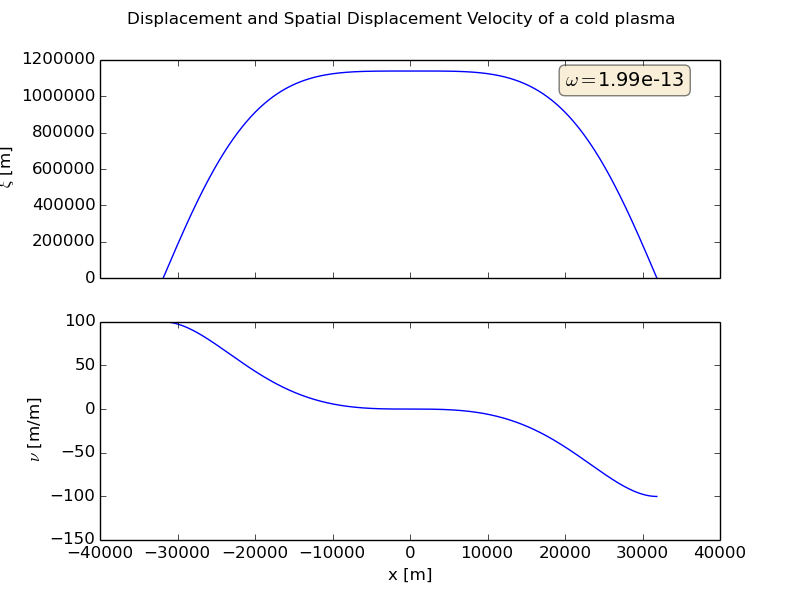
\includegraphics[width = 0.45\linewidth] {../source/wave19950}
    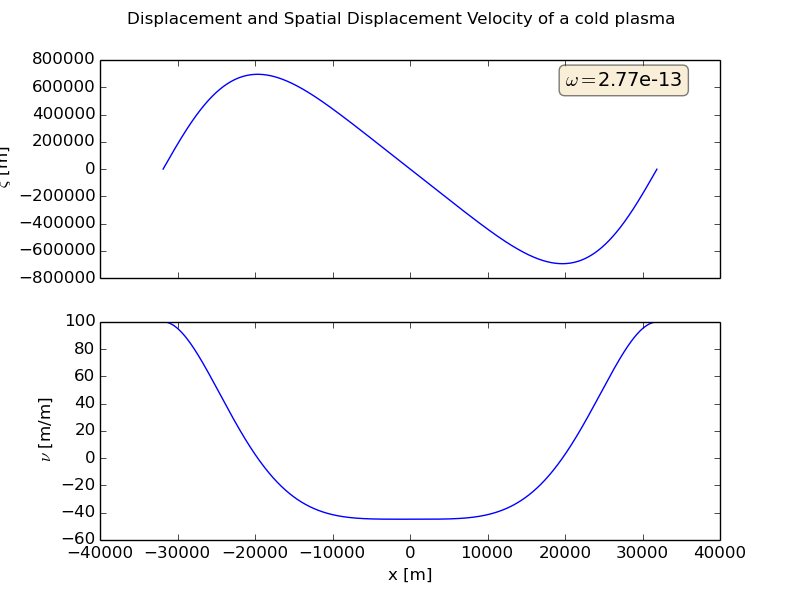
\includegraphics[width = 0.45\linewidth] {../source/wave27650}
    \caption{The first two harmonic waves, of plasma displacement, in a spatially varying magnetic field. The figure on the left has a frequency of \(\omega_1 =1.99\times 10^{-13} \si{\per \second}\), while the figure on the right has the frequency \(\omega_2 =2.77\times 10^{-13} \si{\per \second}\).}
    \label{fig:waves}
  \end{figure}

  We ran the simulation integrating over \(10^6\) spatial steps in the simulations, figures showing the displacement and the displacement velocity of the first two harmonics is shown in \cref{fig:waves}. The first two harmonics were found at the frequencies \( \omega_1 = 1.995 \times 10^{-13} \si{\per \second} \) and \( \omega_2 = 2.765\times 10^{-13} \si{\per \second} \) and it should be noted that the second harmonic is not a integer multiple of the first harmonic, which is also true for the higher harmonics. This is because wave speed is varying over the domain.

  The frequencies tried out had a resolution of \(\Delta\omega = 10^{-16}\), and there are some systematic uncertainties in the integration method that could cause uncertainties in the frequency values.
    
      

\appendix
\section{Comments regarding the exercise}
      \begin{itemize}
        \item Isn't it a harmonic frequency when  \(\nu(-5R_e) = 100 \si{\meter\per\second}\) and \(\nu(5R_e) = -100 \si{\meter\per\second}\) as well?
        \item At \(x = 0\) the magnetic field and mass density approaches \(\infty\), that could cause some trouble with the numerical method. I just truncated it to a high value around \(x=0\).
          Numpy handles it by giving it by giving a really high number of the spatial mesh has a point at \(x=0\), so it works, but I think trimming it is safer if we don't want any overflow instances.
        \item I liked the find by trial and error approach. Fun way to approach a kinda hard problem.
        \item The frequencies I found were very low, compared to the proposed \(0.01\) start. Do I have a serious order of magnitude error somewhere? The displacement numbers also seemed quite high compared to the domain of the wave.
        \item The units on the boundary displacement velocities, \([\si{\meter\per\second}]\) doesn't make sense. It's x-derivative should be in length \([\pdv{\nu}{x}] = [\frac{L/T}{L}] = [T^{-1}]\), \(100\) also sounds abit high when we are covering a distance in the kilometer scale
        \item Good values: Spatial resolution \(10^6\) and frequency on the order \(10^{-13}\)
      \end{itemize}


\section{Code}

  \label{sec:code}
      \lstinputlisting{../source/wave.py}

      

\end{document}